\documentclass{article}[jsarticle]
\usepackage[T1]{fontenc}
\usepackage[dvipdfmx]{hyperref}
\usepackage{lmodern}
\usepackage{latexsym}
\usepackage{amsfonts}
\usepackage{amssymb}
\usepackage{mathtools}
\usepackage{nccmath}
\usepackage{amsthm}
\usepackage{multirow}
\usepackage{graphicx}
\usepackage[dvipdfmx]{color}
\usepackage{wrapfig}
\usepackage{here}
\usepackage{float}
\usepackage{ascmac}
\usepackage{url}
\usepackage{listings}
\usepackage{xcolor}
\usepackage{pifont}

\lstset{
    basicstyle=\ttfamily\color{white},
    numbers=none,  % Line numbers
    numberstyle=\tiny\color{white},
    numbersep=5pt,
    tabsize=2,
    extendedchars=true,
    breaklines=true,
    keywordstyle=\color[rgb]{0.58,0.00,0.83},
    stringstyle=\color[rgb]{0.81,0.36,0.00},
    identifierstyle=\color{white},
    commentstyle=\color[rgb]{0.34,0.62,0.16},
    rulecolor=\color[rgb]{0.5,0.5,0.5},
    xleftmargin=0.1cm,    % Left margin
    xrightmargin=0.1cm,   % Right margin
    language=python,
    backgroundcolor=\color[rgb]{0.13,0.13,0.13},
    showspaces=false,
    showstringspaces=false
}



\title{特別研究3 研究報告書}
\author{高林秀 \\ 三宅研究室 博士前期課程2年 \\ V-CampusID : 23vr008n}
\date{\today}

\begin{document}

\maketitle

\begin{abstract}
    \noindent
    本稿は2024年度特別研究3の研究報告書である。前半は研究テーマの概要と説明を、後半は7月31日現在の研究進捗状況を報告するものである。\par
    \noindent
    特別研究3(以下、本研究と呼称)では、昨年度特別研究2まで行っていた「自律航行ドローンによる物資輸送アプローチの検討」から研究課題を変更し、
    『津波避難誘導の「マルチエージェント強化学習」とドローンによるアプローチの検討』とした。\par 
    \noindent
    % TODO本稿内容の要約
\end{abstract}

\tableofcontents

\section{研究課題について}
本章では、本研究における研究課題の説明と、背景、新規性、最終目標について述べる。
\subsection{概要説明}
\paragraph{研究課題}
\begin{center}
    \textbf{津波避難誘導の「マルチエージェント強化学習」とドローンによるアプローチの検討}
\end{center}
以下、本研究のポイントをまとめる。
\begin{itemize}
    \item 大規模な群衆の津波避難誘導をマルチエージェント強化学習により最適化、機械化を目指す.
    \item 津波避難タワーや津波避難ビルへ避難者を誘導し、制限時間以内で避難率の最大化を目指す
    \item MARL、ゲームAIの災害対応への応用可能性の検証。
\end{itemize}
観光地や沿岸部地域における津波避難の誘導を行うエージェントモデルをマルチエージェント強化学習(以下、MARL)により構築することを目的とする。\par
エージェントはドローンとし、大規模な群衆を複数のドローンによる誘導を行うことで、避難率の最大化を目指す。\par
また、シミュレーションで構築した強化学習モデルを組み込んだ実機でのプロトタイプ制作を行い、実際の運用時における課題や問題点を洗い出す。

昨年度特別研究2までは、『自律航行ドローンによる物資輸送アプローチの検討』を行っていたが、以下の事由により研究課題を上記に変更した。
\begin{itemize}
    \item 強化学習によるアプローチの不適切性
    \item 強化学習により、最適化する指標が不明確であり研究課題として成立しない
\end{itemize}

\subsection{研究背景}
本研究を行う背景と意義について述べる。\par 
大きな背景としては、特別研究1および特別研究2で記載した報告書と同じであるため詳細については、そちらを参照されたい。(特別研究1,2の研究報告書については、付録のURLに添付する)。
ここでは、簡潔に記載するに留める。\par

\paragraph{機械化へのニーズ}
津波に限らず、災害時の避難誘導においては二次被害のリスクを大きく伴う。実際、2011年に発生した東日本大震災では、地元住民の避難誘導に当たっていた警察官の方々が多数殉職するなどの被害も起きている。
この実態について、詳しくは後述の\hyperref[sec:research-sec1]{『我が国における津波避難の課題についての調査』}にて取り上げる。 \par
そういった二次被害を無くし、安全に避難誘導を行うための研究が官民連携で、近年盛んに行われている背景がある。
例えば、東日本大震災で大きな津波被害を受けた宮城県仙台市では、自治体と民間企業が連携し、災害発生状況の確認や避難指示を行うドローンの実証実験が2018年に行われた.
\begin{figure}[H]
    \centering
    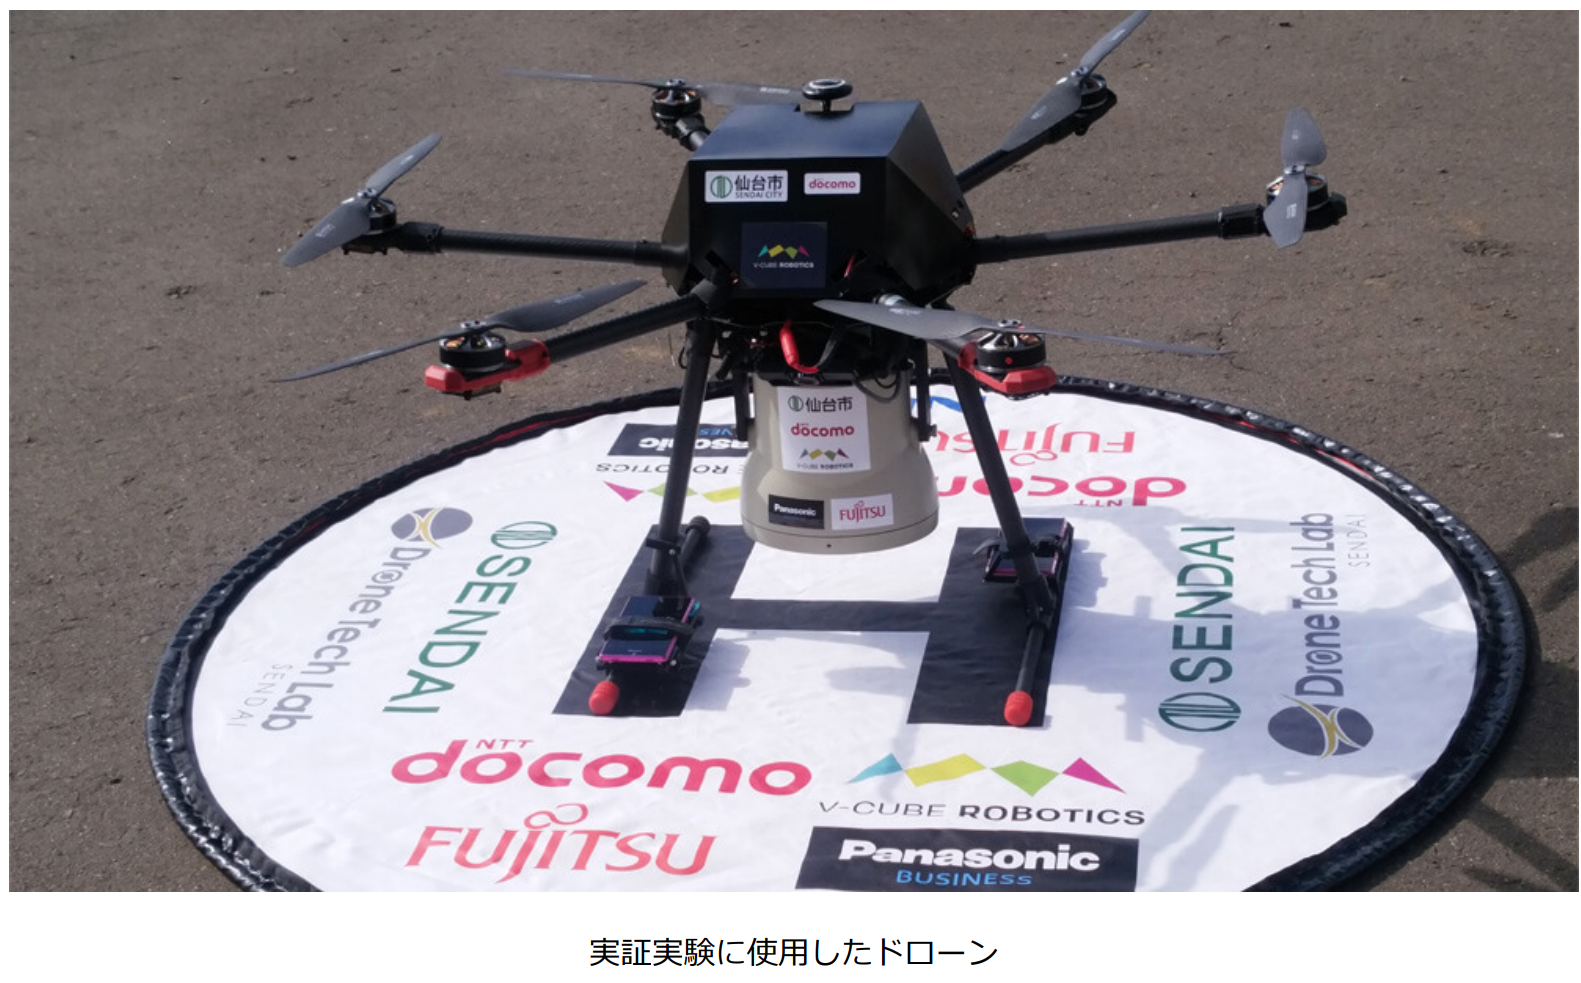
\includegraphics[scale=1.9]{./images/drone1.png}
    \caption{
       仙台市と複数の民間企業の実験で使用されたドローン \\
    【引用元】:富士通ジャーナル『ドローンで津波避難誘導、被災状況をリアルタイムで把握』 2018.04.12
    }
    \url{https://www.fujitsu.com/downloads/JP/microsite/fujitsutransformationnews/journal-archives/pdf/2018-04-12-01.pdf}
\end{figure}

\paragraph{災害対応人材の不足}
災害大国である我が国において, 被災者の捜索, 被害状況の把握,救援物資の現地輸送といった対応は, 迅速かつ効率的に行われなければならない.
しかし近年, そのような災害対応を一任務とする, 自衛隊員の人材が不足している,あるいは今後さらに不足する事態が予想されている。
また、近年その人材不足を補う事に加え


\subsection{新規性・最終目標}
\section{これまでの取り組み}
\subsection{調査関係}
\subsubsection{我が国における津波避難の課題についての調査}
\label{sec:research-sec1}
\subsubsection{先行研究, 類似研究の調査}
\subsubsection{実機実験に向けた調査}
\subsection{シミュレーション・実験関係}
\subsubsection{簡易シミュレータの開発}
\subsubsection{都市モデルでのシミュレーション}
\section{現在の進捗状況}
\subsection{進捗状況まとめ}
\subsection{現在の課題}
\section{修士論文に向けて}
\appendix

\end{document}